\documentclass{article}
\usepackage[margin=2.5cm]{geometry}
\usepackage{graphicx}
\usepackage{units}
\usepackage{amsmath}
\usepackage{multirow}

\usepackage{hyperref}
\hypersetup{colorlinks=true,linkcolor=black,citecolor=black,urlcolor=black}
\urlstyle{same}

\renewcommand{\topfraction}{0.9}    % max fraction of floats at top
\renewcommand{\bottomfraction}{0.8} % max fraction of floats at bottom
\renewcommand{\textfraction}{0.07}  % allow minimal text w. figs

\title{Overcoming confounding plate effects in differential expression analyses of single-cell RNA-seq data}
\author{Aaron Lun}

\begin{document}
\maketitle

\section{Introduction}
Single-cell RNA sequencing (scRNA-seq) is increasingly being used to study molecular biology at the cellular level.
RNA is isolated from individual cells and reverse-transcribed into cDNA fragments that are sequenced using massively parallel technologies \cite{stegle2015computational}.
Mapping of the sequence reads to a reference genome allows quantification of gene expression in each cell, based on the number of reads counted into each gene.
The count data can then be analyzed to identify cell subtypes by clustering on the gene expression profiles;
    to identify highly variable genes contributing to cell-to-cell heterogeneity;
    and to identify differentially expressed (DE) genes between groups of cells.
The ability to assay expression profiles for individual cells provides scRNA-seq studies with biological resolution that cannot be matched by bulk RNA-seq experiments on cell populations.
This comes at the cost of high technical noise, due to the difficulties in sequencing low RNA quantities.

Most existing scRNA-seq protocols are based either on microwell plates \cite{picelli2014full} or microfluidics systems like the Fluidigm C1 \cite{pollen2014low}.
In the former, cells are placed into individual wells, typically with automated approaches such as fluorescently activated cell sorting (FACS).
The entire plate is processed to generate sequencing libraries for all cells at once.
In the latter, individual cells are captured in separate reaction chambers within the C1 chip 
    (for simplicity, each chip will be treated as being equivalent to a plate in the following text).
All cells on each chip are then simultaneously processed into libraries.
Each plate or chip can only handle a limited number of cells, so data is usually generated for multiple plates across several biological conditions. 
All cells on each plate typically come from the same population (e.g., culture, embryo, animal) of a single biological condition.
Multiple plates are used for cells from replicate populations of the same condition.

The experimental design described above is motivated largely by practicality.
It is logistically simpler to track and process cells when each plate corresponds to one population of one condition, compared to partitioning the plate into separate conditions.
For example, FACS is typically performed such that all cells on a plate are derived from the same gates, i.e., from the same subpopulation.
In the C1, cells are captured randomly into reaction chambers such that the identity of the cell in each chamber cannot be pre-specified.
Ambiguity in determining the condition for each cell is avoided by only using cells from the same condition on each chip.
However, this design can result in a ``plate effect'' where uncontrollable experimental variables have a consistent effect for all cells on each plate but a variable effect across different plates. 
These variables can be technical in origin, such as differences in library preparation or sequencing between plates; 
    or biological, due to inherent variability in gene expression between the replicate populations on different plate.

One common analysis of scRNA-seq data involves identifying DE genes between groups of cells.
This does not strictly require single-cell resolution, and is more conventionally performed with bulk data.
Nonetheless, there are some benefits to using single-cell data, especially for situations involving rare cells and quality control.
It is also more practical to perform the DE analysis on existing scRNA-seq data compared to generating bulk RNA-seq data exclusively for this purpose.
The DE analysis itself is performed using software packages such as edgeR \cite{robinson2010edgeR} and DESeq \cite{anders2010differential}, which were designed for bulk data;
    or with methods such as monocle \cite{trapnell2014dynamics}, which were designed explicitly for single-cell data.
Putative DE genes are defined as those that exhibit significant differences in the average counts between two or more biological conditions of interest.

The presence of plate effects complicates the parametrization of the experimental design for the DE analysis.
Such effects are obviously undesirable as they result from uncontrolled experimental variability.
This increases the estimated variance and reduces the power to detect DE genes.
However, they cannot be easily removed during the statistical modelling.
This is because the plate effect is confounded by the conditions of interest.
At the most extreme, consider a situation involving one plate for each condition.
Changes in gene expression due to the plate effect will be indistinguishable from genuine DE between conditions.
This problem is still present with two or three plates per condition, where plate-to-plate variability may explain some or all of the apparent DE between conditions.
In lieu of a sensible method to remove plate effects, most studies have simply ignored them and treated cells from different plates as direct replicates \cite{kolod2015single,trapnell2014dynamics,avraham2015pathogen}.
This may not be statistically rigorous as the variability across plates and cells will not be modelled properly.

This article demonstrates that plate effects must be handled properly to maintain the statistical validity of a DE analysis.
In a simple simulation, all analyses that ignored the plate effects failed to control the type I error rate.
This was caused by the presence of correlations between cells on each plate during variance estimation.
To avoid detection of spurious DE, a summation approach was proposed whereby counts for all cells on each plate were summed prior to analysis.
This restored control of type I error across a range of simulation scenarios, without compromising DE detection power.
Similar effects were observed in real data where summation resulted in substantial changes to the number and ranking of genes in the DE list.

\section{Plate effects result in false positives in a DE analysis}

\subsection{Description of the experimental design and analysis strategies}
Consider an experimental design consisting of multiple biological conditions of interest.
Each condition consists of cells sorted onto multiple plates, where all cells on a single plate correspond to a single condition.
As previously mentioned, this is not an uncommon setup due to the logistics of the experimental protocol, e.g., cell sorting onto a plate with FACS, cell capture with the C1.
Further assume that a plate effect exists in the data set, whereby the expression of each gene in all cells of a given plate is modified in a gene- and plate-specific manner.
Consideration of gene specificity in the plate effects is motivated by biological variability across cell populations, 
    given that all cells on each plate are often derived from a separate population.
More precisely, the observed read count for gene $i$ in cell $j$ in plate $k$ of condition $l$ is distributed as 
\[
    y_{ij} | \delta_{ik}  \sim X_{ik}
\]
where $\delta_{ik}$ is the plate-specific effect for this gene.
$X_{ik}$ is some random variable such that 
\[
    E(X_{ik}) = \delta_{ik}\mu_{il}
\]
where $\mu_{il}$ is the expected read count for condition $l$. 
Any references to the conditional distribution, variance or mean will refer to the corresponding attributes of $X_{ik}$.
%In other words, the conditional distribution of $y_{ij}$ given $\delta_{ik}$ is defined as $X_{ik}$.
The plate effect $\delta_{ik}$ is sampled from some independent distribution $Y$ where $E(Y) = 1$.
This ensures that $E(y_{ij}) = \mu_{il}$, consistent with the definition of $\mu_{il}$.

One aim of the data analysis for this experiment is to identify DE genes between conditions.
This is complicated by the presence of the plate effects.
These effects cannot be removed by scaling normalization 
    -- they vary for each gene and cannot be negated by global scaling of the counts for each cell.
The plate effects are also confounded by the biological condition, as previously described.
A fold-increase in $\delta_{ik}$ cannot be distinguished from a matching increase in $\mu_{il}$, based solely on the counts for a single plate.
Any attempt to remove the former will affect detection of genuine DE in the latter.
Even with multiple plates, this problem is present as stochastic increases in $\delta_{ik}$ for all $k$ in $l$ can explain part or all of the observed DE.

A common strategy ignores the plate effects and treats the cells from different plates as direct replicates.
The estimated variance will include the conditional variance between cells on a given plate, i.e., var$(X_{ik})$, as well as that of $\delta_{ik}$ between plates.
Methods can then be applied to detect DE between conditions, using software designed for bulk RNA-seq data (e.g., DESeq) or with dedicated single-cell methods (e.g., monocle).
This approach has been used in a number of scRNA-seq studies to detect DE across plates or chips \cite{kolod2015single,trapnell2014dynamics,avraham2015pathogen}.
However, it is not clear whether statistical rigor is maintained when plate effects are simply ignored.

% Trapnell paper uses one C1 chip for each timepoint.
% Kolod...'s paper has multiple chip for each serum condition.
% Avraham's paper has 192 cells for the Salmonella exposed, and 96 for unexposed; this must be different plates.

\subsection{Simulating plate effects to evaluate analysis methods}
A simple simulation is used to test the performance of the analysis when plate effects are ignored.
Let the count for each gene in each cell follow a negative binomial (NB) distribution, conditional on the plate effect.
In other words, $X_{ik}$ represents a NB-distributed random variable with a mean of $\delta_{ik}\mu_{il}$ and a dispersion of $\varphi_i$.
The size of $\varphi_i$ determines the variance of the conditional distribution represents the magnitude of the cell-to-cell heterogeneity within each plate.
The plate effects themselves are sampled from a log-normal distribution, i.e., $Y = \ln \mathcal{N}(\nicefrac{-\sigma^2}{2}, \sigma^2)$.
This parametrization ensures that $E(Y)=1$, as originally defined.

Simulated data was generated for 10000 genes across two conditions, each consisting of 3 replicate plates with 50 cells in each plate.
The expected read count for each condition was set to $\mu_{il}=\mu_{i0}$, where $\log \mu_{i0}$ was sampled from a uniform distribution over the interval (3, 8).
This captures the spread of abundances for different genes in real data. 
For each gene $i$, the NB dispersion was defined according to the mean, i.e., 
\[
    \varphi_i = \frac{1}{2} + \frac{100}{\mu_{i0}} 
\]
to represent the decreasing mean-dispersion trend observed in real data.
Large values of $\varphi_i$ are also consistent with high technical and biological variability in scRNA-seq counts.
Finally, $\sigma^2$ was set to a value of 0.5 to represent a strong plate effect.
Simulations were repeated with $\sigma^2=0$ (i.e., no plate effect) as a control. 

\subsection{Implementation of DE analysis methods}
DE analyses of the simulated data were performed using edgeR v3.12.0, DESeq2 v1.10.0 \cite{love2014moderated}, voom \cite{law2014voom} in limma v3.26.3, 
    monocle v1.4.0 and MAST v0.931 \cite{finak2015mast}.
edgeR, DESeq2 and voom are methods designed for analyses of bulk RNA-seq data.
edgeR and DESeq2 model counts with NB distributions, while voom uses a normal distribution to model log-counts per million (log-CPMs) with precision weights.
monocle and MAST are explicitly designed for analyzing scRNA-seq data and operate on pre-processed expression values.
In all methods, the experimental design was parametrized as a one-way layout with two conditions.
All cells within each condition were treated as replicate samples -- the plate of origin within each condition was ignored.

For edgeR, analyses were performed with and without empirical Bayes (EB) shrinkage.
In the first analysis, an abundance-dependent trend was fitted to the NB dispersions, 
    and the trended NB dispersion was used to fit a generalized linear model (GLM) for each gene \cite{mccarthy2012differential}.
The GLM deviance was used to estimate the quasi-likelihood (QL) dispersion for each gene, 
    which was stabilized by robust EB shrinkage towards another mean-dispersion trend \cite{lund2012detecting}.
DE testing between conditions was performed using the QL F-test.
In the second analysis, the NB dispersion was estimated for each gene individually.
This was used directly to fit the GLM for each gene, and DE testing was performed using the likelihood ratio test (LRT).

For voom, counts were converted to log-CPMs and precision weights were computed from a fitted mean-variance trend.
Log-CPMs and weights for each gene were used to fit a linear model.
Variances were stabilized by EB shrinkage, and genes were tested for DE between conditions using a moderated $t$-test.
This analysis was also repeated after using the duplicateCorrelation function to estimate the correlation between cells on the same plate.
The consensus correlation was incorporated into the variance estimation by blocking on the plate of origin during fitting of the linear model.
DE testing was then repeated on this refitted model.

For DESeq2, the NB dispersion was estimated for each gene and a mean-dispersion trend was fitted across genes.
A normal prior was applied to the log-dispersions for all genes, and the maximum \textit{a posteriori} estimate of the NB disperison was obtained for each gene.
The estimated dispersion was used to fit a GLM to the counts for each gene.
Finally, DE testing was performed between conditions using the Wald test.

For edgeR and voom, normalization was performed prior to modelling using the trimmed mean of M-values (TMM) method \cite{robinson2010scaling}.
For DESeq2, normalization was performed using size factors.
This step is not strictly necessary in this simulation, given that library-specific biases have not been introduced and all cells have the same library size.
Nonetheless, normalization is included as part of the standard analysis.

For monocle, counts were transformed into CPM values that were considered to be roughly log-normal.
These were used for DE testing between conditions with the LRT in the differentialGeneTest function.

For MAST, counts were log-transformed after adding a prior count of 1.
All libraries were of the same size, and all genes were of the same length, 
    so the log-counts are effectively equivalent to the log-transcripts per million used in the original description of the algorithm \cite{finak2015mast}.
A hurdle model was fitted to the log-counts using the biological condition as the factor of interest and the number of non-zero counts in each library as a covariate.
The fitting method was set to ``bayesglm'' and empirical Bayes shrinkage was turned on with the ``MLE'' method and the ``H1'' model.
DE genes between conditions were identified using the LRT.

In all analyses, the null hypothesis is true for each gene $i$ as $\mu_{il}$ is constant for both conditions.
Any rejections of the null represent type I errors, i.e., false positives.
For a specified type I error rate $\alpha = 0.01$, the observed error rate was defined as the proportion of all genes with a $p$-value below $\alpha$.
This was averaged across 10 simulation iterations to obtain a stable estimate of the observed type I error rate for each method. 
A method was considered to be liberal if its observed error rate in the simulation was above the specified $\alpha$.
Note that this evaluation is only possible for methods that compute $p$-values for each gene -- 
    Bayesian methods \cite{vallejos2015basics,kharchenko2014bayesian} are not comparable as they generate posterior probabilities, and so are not tested here.

% BASiCS requires spike-ins, that the other methods don't use, so it's not entirely comparable.
% Kharchenko's method generates z-scores and MLEs, but no p-values.

\subsection{Type I error control is lost by all methods}
The observed type I error rate exceeds the specified threshold in all methods (Figure~\ref{fig:platefail}).
In all methods except for voom with correlations, the discrepancy between the observed and specified rates is greater than an order of magnitude.
This liberalness is attributable to the plate effect, rather than any inherent fault with the methods.
In the control simulation with $\sigma^2=0$, the observed rates for all methods are substantially closer to the threshold, if not below it.
These results suggest that DE analyses will perform poorly if the plate effect is simply ignored.
Loss of type I error control will result in an unacceptable number of false positives in the final set of DE genes.
This is equally applicable to the false discovery rate (FDR), given that control of the FDR depends on proper control of the type I error when the null hypothesis is true.

\begin{figure}[tbp]
\begin{center}
\includegraphics[width=0.48\textwidth,trim=0mm 0mm 0mm 10mm,clip]{failsim_with_raw.pdf}
\includegraphics[width=0.48\textwidth,trim=0mm 0mm 0mm 10mm,clip]{failsim_without_raw.pdf}
\end{center}
\caption{
    Observed type I error rates for each method on simulated data, in the presence (left) or absence (right) of a plate effect.
    Error rates are shown on a log scale and represent the average across 10 simulation iterations.
    Each error bar represents the standard error of the log-average rate.
    The threshold of 0.01 is represented by the red dotted line.
    Only one iteration was used for monocle due to its running time.
}
\label{fig:platefail}
\end{figure}

Loss of type I error control is caused by correlations between cells on the same plate.
Most DE analysis methods assume that replicate samples (i.e., cells) are independent.
This is not the case when a plate effect is present -- all cells on the same plate will be positively correlated, as expression is modified by the same plate effect.
These correlations reduce the amount of information in the data set, as cells on the same plate are effectively redundant.
However, most methods do not consider the correlations and will overstate the amount of information for variance estimation.
This results in overconfident inferences and liberalness.

The problem can also be described in terms of the residual degrees of freedom (d.f.) that are available to estimate the variance.
The simulation uses an experimental design with $6 \times 50 =  300$ cells and two coefficients in a one-way layout.
If all cells were truly independent -- as is assumed by most methods -- this design would provide 298 residual d.f. 
At the other extreme, consider the scenario where all cells on a plate are completely correlated.
This means that there are only six independent samples (one cell per plate, as all other cells on each plate are redundant) and only four residual d.f.
This is substantially smaller than the 298 d.f.\ expected by each method, which is problematic.
For example, the use of edgeR with the LRT assumes that sufficient residual d.f.\ are present to estimate the dispersion for each gene separately,
    without requiring EB shrinkage to share information between genes.
This is no longer justifiable if only four d.f.\ are available.

It is worth pointing out that the voom with correlations method explicitly accounts for the intra-plate correlations between cells.
This method exhibits the best performance of all tested methods in the presence of a plate effect (Figure~\ref{fig:platefail}),
    i.e., the observed type I error rate is closest to the specified threshold.
Nonetheless, voom with correlations is still liberal.
This is attributable to the inadequacy of the normal model for highly discrete counts, particularly in scRNA-seq where low-abundance genes have many zero counts.

\subsection{Alternative analysis strategies are unpalatable}
Simply ignoring the plate effects results in unacceptable loss of control.
However, the obvious alternatives are not without their own difficulties.
One approach would be to introduce blocking factors for the plates into the model.
In a log-link model similar to that used in edgeR and DESeq, this is equivalent to setting
\[
    \beta_{ij} = \beta_{il} + \beta_{ik} + o_{ij}
\]
where $\beta_{ij}$ is the log-expression for gene $i$ in cell $j$, $\beta_{il}$ is the average log-expression for condition $l$, 
    $\beta_{ik}$ is the plate effect for plate $k$ and $o_{ij}$ is a normalization offset.
The intention is that $\beta_{ik}$ will absorb differences in $\delta_{ik}$ between $k$, thus eliminating the plate effect.
However, $\beta_{ik}$ will also absorb differences in $\mu_{il}$ between conditions.
This will eliminate genuine DE and reduce detection power.
The same problem is observed for methods like ComBat \cite{johnson2007adjusting} when they are applied to remove confounding plate effects prior to a DE analysis.
In addition, the design matrix will not be of full column rank when plate blocking factors are added, i.e., not all coefficients are estimable.
This cannot be resolved without altering the interpretation of $\beta_{il}$ such that it no longer represents the condition average.
For example, one could set $\beta_{ik}=0$ for the first plate in each condition, 
    but $\beta_{il}$ would then represent the log-expression of that first plate alone rather than the average of all plates for $l$.
As such, it would not be sensible to treat differences in $\beta_{il}$ as DE between conditions.

A more elegant model involves orthogonal plate and condition terms.
For a simple experimental design involving two plates in two conditions ($k=1,2$ for $l=1$, $k=3,4$ for $l=2$), this can be parametrized as
\[
    \beta_{ij} = \beta_{il} + 
    \begin{cases} 
        \beta_{il0} & \mbox{if $k$ is odd} \\
        - \beta_{il0} & \mbox{if $k$ is even}
    \end{cases}
    + o_{ij}
\]
where $\beta_{il0}$ represents the plate-specific residual around the mean log-expression $\beta_{il}$ for each condition.
Differences in $\mu_{il}$ between conditions will be detected as differences in $\beta_{il}$, 
    while differences in $\delta_{ik}$ within conditions will be captured by $\beta_{il0}$ and removed.
The problem with this setup is that the variability of the plate effect is absorbed by $\beta_{il0}$.
This means that it is not incorporated into the variance estimate within the DE analysis, which only considers the conditional variance of the counts within each plate.
If one were to generate new data for the same experimental design, one would expect a different set of values for the plate effects.
Failure to account for the variability of $\delta_{ik}$ across plates will compromise the reproducibility of the results.
Indeed, application of this approach in the previous simulation (by modifying the design matrix appropriately and applying QL edgeR)
    results in an observed type I error rate of 0.55 at a specified threshold of 0.01.

The most sophisticated approach uses a mixed model with fixed effects for the conditions and random effects for the plates.
This accounts for plate-to-plate variability while considering the correlations between cells on each plate.
However, mixed models are difficult to implement and are not supported by most existing methods for analyzing genomic data, e.g., edgeR.
One can instead use general statistical methods for mixed modelling such as those in the lme4 package \cite{bates2015fitting}.
To test this approach, the glmer.nb function in lme4 v1.1-10 was used to fit a NB generalized linear mixed model to the simulated counts for each gene.
This still was not able to control type I error rate, yielding an observed rate of 0.032 at a threshold of 0.01.
Model fitting was also more time-consuming, taking several hours to run for a single simulation iteration compared to several minutes for edgeR.
Furthermore, the amount of information for estimating the variability of the plate random effect is determined by the number of plates, not the number of cells.
In data sets with few plates, little information is available for each gene -- this reduces the stability of the variance estimates and the power to detect DE.
This is not an issue for genomics methods like edgeR that share information across genes.

\section{Improved performance with summation across cells in each plate}

\subsection{Error control can be restored by summing over cells}
A simple solution presents itself for restoring error control in the presence of plate effects.
Firstly, the counts for each gene are summed across all cells within each plate.
These count sums are then supplied to the DE analysis software, where the plates themselves are treated as replicate samples for each condition.
This ensures that the analysis does not overestimate the residual d.f.\ of the design.
Correlations between samples are no longer present when plates are considered instead of cells, given that the plate effect is assumed to be independent between plates.
Summation has the additional benefit of increasing the size and precision of the counts.
This makes the data more amenable for analysis with methods designed for bulk data.

Summation substantially reduces the liberalness of the DE analysis methods in the simulation (Figure~\ref{fig:platesum}).
This is attributable to the proper consideration of the true number of residual d.f.\ in the experimental design.
Some mild liberalness is still observed for edgeR and DESeq2.
This is due to the fact that the counts are not truly NB-distributed, which results in some inaccuracy during modelling.
voom is inherently more conservative \cite{law2014voom}, which results in lower observed rates and restoration of type I error control.
The other methods are not used here, for various reasons -- voom with correlations is not necessary as the replicate plates are independent;
    monocle is designed for per-cell data rather than summed per-plate counts;
    and for edgeR without EB shrinkage, there are insufficient residual d.f.\ to stably estimate the dispersion.

\begin{figure}[tbp]
\begin{center}
\includegraphics[width=0.48\textwidth,trim=0mm 0mm 0mm 10mm,clip]{failsim_with_sum.pdf}
\end{center}
\caption{
    Observed type I error rate for each method after summation in simulations with a plate effect.
    Error rates are shown on a log scale and represent the average across 10 simulation iterations.
    Error bars represent standard errors, and the threshold of 0.01 is represented by the red dotted line.
}
\label{fig:platesum}
\end{figure}

\subsection{Summation does not compromise DE detection power}
It should be stressed that summation of counts does not change the nature of the underlying changes in expression.
In a DE analysis, the average expression of each gene is compared between two or more conditions.
This is true regardless of whether those conditions contain replicate cells or replicate plates 
    (scenarios involving differing numbers/sizes of cells per plate will be considered in the next section).
In general, summation only affects the estimation of the variance rather than that of the effect size, i.e., the log-fold change.

This can be demonstrated with a simulation involving genes that have genuine DE between conditions.
DE was introduced for 1000 randomly selected genes by setting $\mu_{il_1} = 3\mu_{il_2}$ for conditions $l_1$ and $l_2$, i.e., a 3-fold increase in expression in the first condition.
This was repeated for a separate set of 1000 genes by setting $\mu_{il_2} = 3\mu_{il_1}$.
The balanced addition of DE genes ensures that composition biases \cite{robinson2010scaling} are not introduced between samples.
Simulated data was then generated in the presence of a plate effect (i.e., $\sigma^2=0.5$), as previously described
Analyses with DESeq2, limma and voom were performed on the single-cell and summed counts.
A receiver-operating-characteristic (ROC) curve was constructed for each analysis by defining the true and false positive rates as the proportion of DE and non-DE genes that were detected, respectively.
For each method, the ROC curve obtained with the analysis on summed counts is near-identical to that obtained with single-cell counts (Figure~\ref{fig:roc}).
This indicates that detection power is not affected by summation.

\begin{figure}[tbp]
\begin{center}
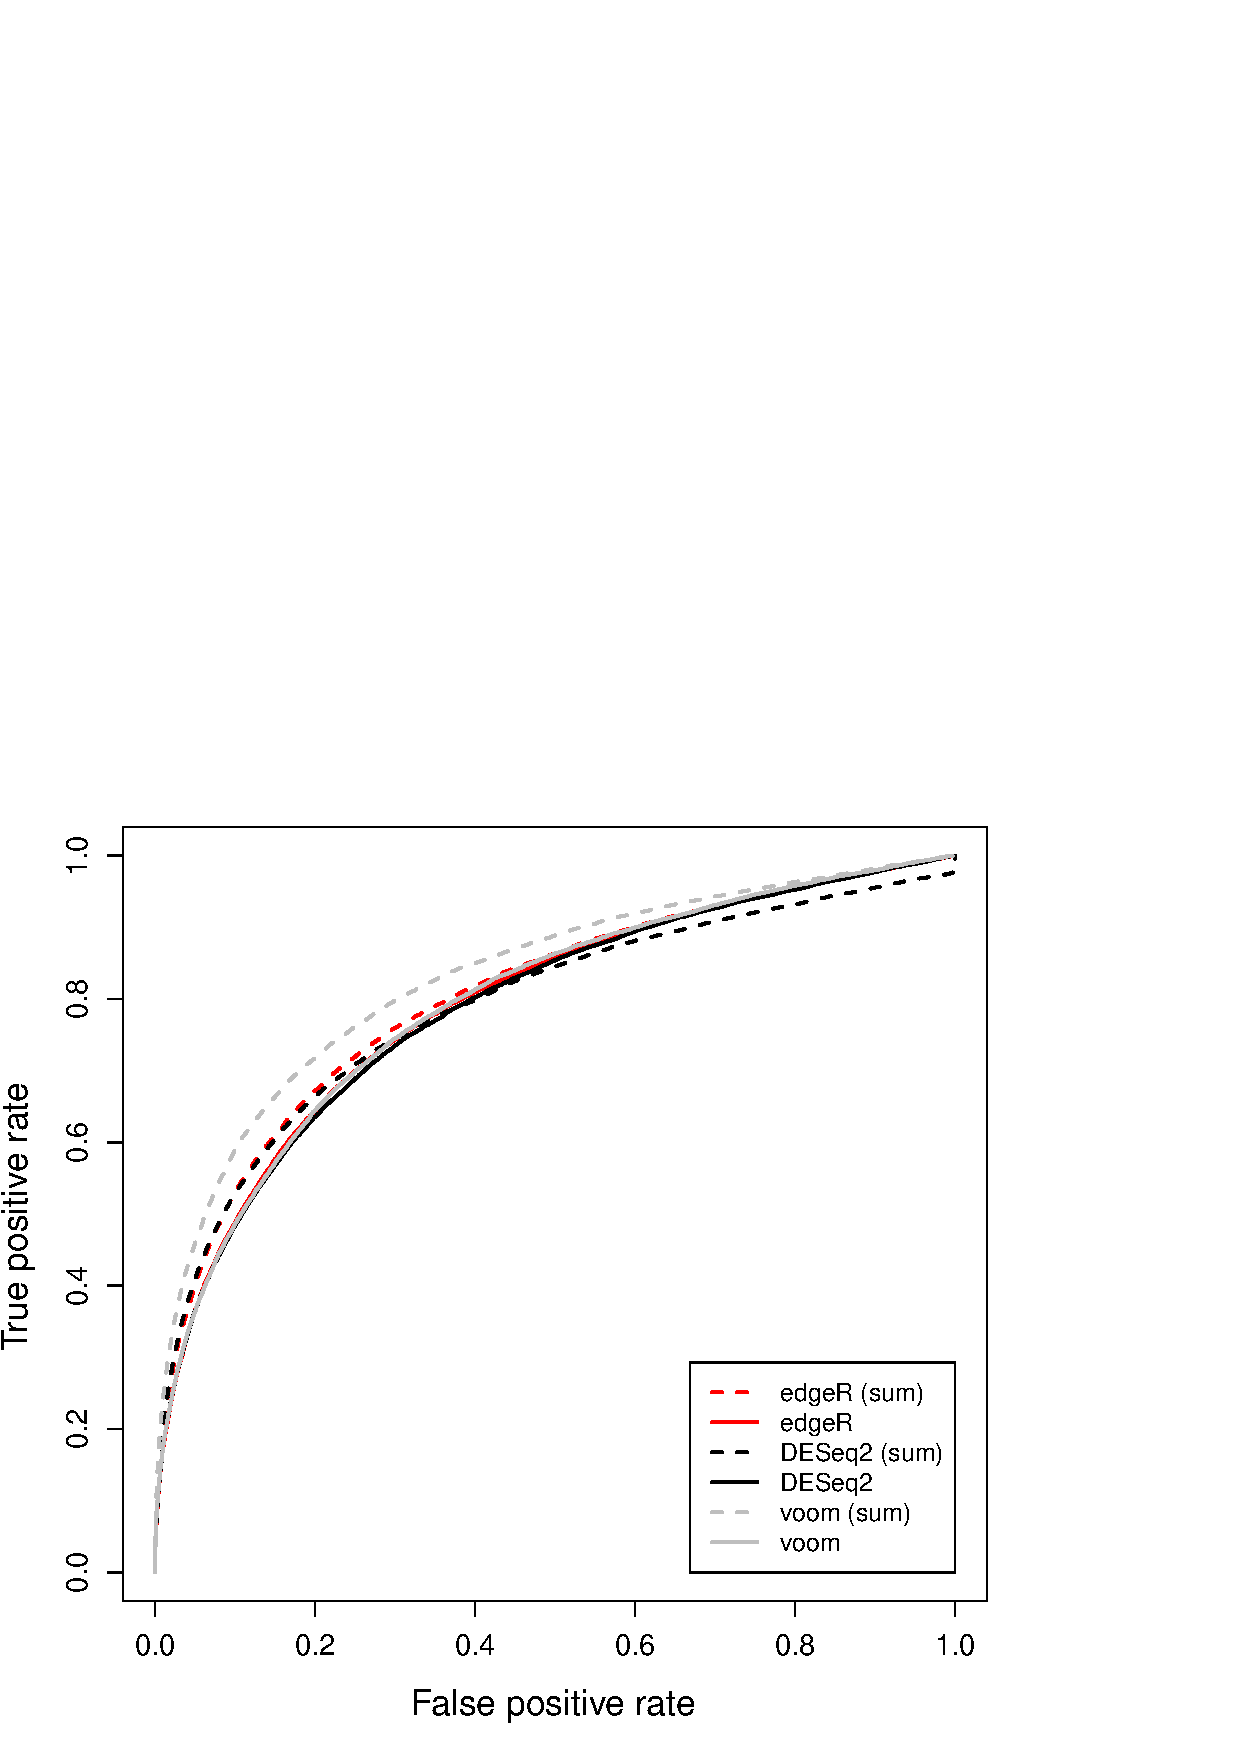
\includegraphics[width=0.48\textwidth]{power_with.pdf}
\end{center}
\caption{
    ROC curves for each analysis method on simulated data with a plate effect and genuine DE, for both single-cell (full) and summed counts (dashed).
    Curves are shown for DESeq2 (black), voom (grey) and edgeR (red).
    Each curve represents the average result of 10 simulation iterations.
}
\label{fig:roc}
\end{figure}

\subsection{Justifying summation in a single-cell study}
Despite the obvious improvement in performance, the summation strategy may not have unqualified appeal.
After all, it seems to contradict the purpose of a scRNA-seq study. 
Why would one bother to sequence the transcriptome of individual cells, only to add the counts together during the analysis?
The use of summed counts is equivalent to performing bulk sequencing on the pooled population, which would be technically easier to undertake and analyze.
In fact, this apparent contradiction is relevant to all DE analyses of scRNA-seq data where average expression levels are compared between pre-defined groups of cells.
Such averages could be obtained directly with bulk sequencing of the groups, rather than of single cells.

The resolution of this contradiction is based on the ability of single-cell approaches to characterize and define the groups prior to the DE analysis.
Rare cells can be profiled in scRNA-seq that cannot be obtained in sufficient numbers for bulk sequencing.
Low quality libraries or contaminating cells can be identified and removed from each group to avoid interfering expression patterns.
Groups can also be empirically identified based on gene expression patterns (though this requires some care to maintain statistical rigour in the subsequent DE analysis).
Obviously, it is not mandatory to use the summed counts exclusively 
-- single-cell counts can still be used for other aspects of the analysis, e.g., clustering, identifying highly variable genes.
All of these advantages are lost when RNA sequencing is performed at the population level.

Note that summation across cells in scRNA-seq data is not without precedent.
Jaitin \textit{et al.} pool single-cell expression profiles to obtain a combined vector of subpopulation-level counts for gene clustering \cite{jaitin2014massively}.
Klein \textit{et al.} also pool single-cell counts within each condition prior to a DE analysis between conditions,
    to assess the technical reproducibility of their experimental protocol \cite{klein2015droplet}.
However, the use of summation to restore type I error control in the presence of plate effects has not yet been addressed in the literature.

\section{Error control does not require variance adjustment}

\subsection{Direct summation may yield inconsistent mean-variance relationships}
The simulation used in the previous section describes a situation involving the same number of libraries of the same size on each plate.
A result of this experimental design is that the count sums for all plates are identically distributed for any given gene.
This is statistically convenient as it substantially simplifies the modelling procedure.
However, more realistic data sets will contain different numbers of cells in each plate, as well as different library sizes across cells.
In such scenarios, the count sum for each plate will not be identically distributed.
The most obvious difference is that in the magnitude of the count sum between different plates, 
    but this can be easily corrected by normalizing on the total library size for each plate (i.e., the sum of count sums across genes).
The greater problem is that the count sum for each plate will not follow the same mean-variance relationship.
This will compromise the accuracy of most parametric models.

To illustrate, consider the NB-based simulation framework described in the previous section.
Denote the count sum for gene $i$ in plate $k$ as $s_{ik}$.
Denote the conditional mean of $s_{ik}$ as $E(s_{ik}|\delta_{ik})=N_k \delta_{ik}\mu_{il} = \rho_{ik}$, where $N_k$ is the number of cells in plate $k$.
The sum of independently and identically NB-distributed random variables is itself NB-distributed, 
    such that $s_{ik} |\delta_{ik} \sim \mbox{NB}(\rho_{ik}, \nicefrac{\varphi_i}{N_k})$.
The conditional variance is then
\[
    \mbox{var}(s_{ik} |\delta_{ik}) = \rho_{ik} + \frac{\varphi_i}{N_k}\rho_{ik}^2 \;.
\]
As $\delta_{ik}$ is independent of the other parameters, the total variance of $s_{ik}$ can be written as
\begin{align*}
    \mbox{var}(s_{ik}) &= (N_k\mu_{il})^2\mbox{var}(\delta_{ik}) + N_k\mu_{il} + \varphi_i N_k\mu_{il}^2 E(\delta_{ik}^2) \\
                       &= E(s_{ik})^2 \mbox{var}(\delta_{ik}) + E(s_{ik}) + \frac{\varphi_i}{N_k} E(s_{ik})^2 E(\delta_{ik}^2) 
\end{align*}
where $E(s_{ik})=N_k\mu_{il}$. 
The $\mbox{var}(\delta_{ik})$ and $E(\delta_{ik}^2)$ terms are constant, as is the $\varphi_i$ term.
This means that the mean-variance relationship of $s_{ik}$ will not be identical across $k$ when $N_k$ differs between plates.
Plate-specific differences in library size lead to similar complications, by altering the distribution of each $s_{ik} |\delta_{ik}$.

Data sets with observation-specific mean-variance relationships are not typically considered in most analysis pipelines.
For example, standard edgeR and DESeq2 analyses use a single NB dispersion estimate for each gene.
This defines an identical mean-variance relationship for all counts of the gene, which reduces the accuracy of the model when the relationship varies across counts.
Model inaccuracy is particularly problematic when the variance is consistently underestimated across all plates in a condition.
Such cases will result in loss of error control and detection of spurious DE between conditions.
This may affect the performance of the summation strategy when the numbers of cells and library sizes vary between or within plates.

\subsection{Preserving the mean-variance relationship with quantile adjustment}
One solution to this problem uses quantile adjustment \cite{robinson2008small} to generate Poisson-distributed pseudo-counts.
This exploits the fact that the sum of independently Poisson-distributed variates is itself Poisson-distributed, conditional on the plate effect.
The mean-variance relationship of the pseudo-count sum $\tilde{s}_{ik}$ becomes 
\[
    \mbox{var}(\tilde{s}_{ik}) = E(\tilde{s}_{ik})^2 \mbox{var}(\delta_{ik}) + E(\tilde{s}_{ik}) 
\]
such that it will be identical for all $k$, regardless of the number and size of libraries.
Statistical modelling can then be performed with standard methods that do not consider observation-specific relationships.

The quantile adjustment method models the conditional distribution of each count as a NB distribution.
All cells within a single plate are defined as a separate group in a one-way layout.
For each gene, means are estimated for all cells by fitting a GLM to the counts for that gene.
The mean for each cell accounts for its library size as well as any gene- and plate-specific effects.
A gene-specific NB dispersion is also estimated using standard methods, e.g., with the Cox-Reid adjusted profile likelihood in edgeR \cite{mccarthy2012differential}.
The count for each cell is now modelled by a NB distribution with the estimated mean and dispersion.
The percentile corresponding to each count is computed, and the matching quantile for a Poisson distribution with the same mean is identified.
This quantile is Poisson-distributed and is used as the pseudo-count for each cell.

This method depends on stable estimation of the mean for each cell and the dispersion for each gene.
The latter should not be an issue as there should be sufficient residual d.f. across all cells to obtain a precise dispersion estimate.
Note that the previously mentioned problems with residual d.f. overestimation are not applicable here.
Correlations induced by plate effects are avoided as plate-specific expression is explicitly modelled in the one-way layout.
For the means, stable estimation can be ensured by having sufficient cells per plate.
This is usually the case given that low-quality plates with very few cells would be removed.

\subsection{Direct and quantile-adjusted summation control type I error rates}
The performances of direct and quantile-adjusted summation were evaluated with more complex simulations involving different numbers of cells and library sizes per plate.
Simulated data was generated using the previously described model (i.e., NB-distributed counts and log-normal plate effects), with some modifications.
Briefly, the conditional distribution of $y_{ij}$ was redefined as a NB distribution with mean $\delta_{ik}\theta_{j}\mu_{ik}$.
The $\theta_{j}$ term represents the relative library size for each cell $j$ and is set to unity unless otherwise specified.
The experimental design was also changed such that only two plates were present for each condition.

To assess the effect of different cell numbers, data was simulated for 10 cells in all plates of one condition and 100 cells in all plates of the other condition.
Library sizes were kept constant for all cells in this simulation scenario.
To assess the effect of library size, the number of cells per plate was kept constant at 50.
Three scenarios were tested, by setting $\theta_j=5$ for 20 cells in each plate of one condition (all plates in the other condition were unchanged);
    $\theta_j=10$ for 10 cells; and $\theta_j=20$ for 5 cells.
In all cases, library sizes are only modified for a fraction of cells on a subset of plates. 
This subtlety is necessary because the mean-variance relationship will be preserved between plates if there is a consistent increase in the library size for all cells on a plate, 
    or if there is an increase in the library size for the same proportion of cells on all plates.

The use of two plates in each condition also allows the simulated data set to be permuted.
Specifically, plates can be swapped between conditions such that each condition contains replicate plates with differing numbers of cells (in the first scenario)
    or cells with different library sizes (in the other scenarios).
This swapping procedure generates scenarios where differences between plates occur within conditions, 
    complementing the original simulations where the differences only occur between plates in different conditions.

Direct and quantile-adjusted summation were applied on the simulated data by summing the counts or pseudo-counts for all cells in each plate.
The resulting (pseudo-)count sums were tested for DE between conditions, using the QL framework in edgeR as a representative of the bulk analysis methods.
The observed type I error rate was calculated, and the average rate was computed across 10 simulation iterations.
This was repeated for each scenario described above, before and after swapping replicate plates between conditions.
As a control, the analyses were also performed on simulated data without a plate effect, i.e. $\sigma^2=0$.

Both strategies are able to control the type I error close to the specified threshold (Figure~\ref{fig:complexplate}).
This is despite the presence of differences in the number of cells per plate or the library sizes between cells,
    which would be expected to yield differences in the mean-variance relationship in the summed counts.
The performance of direct summation is attributable to the precision of the count sum when many cells are present on each plate.
When counts are summed across many cells, cell-specific technical noise and biological heterogeneity average out through the law of large numbers.
The conditional variance of the count sum approaches the variance of a Poisson distribution, due to sequencing noise \cite{marioni2008rnaseq} that is common to all samples.
This means that the count sum for each plate will have near-identical mean-variance relationships, as described above for the pseudo-counts.
Any differences in these relationships are quantitatively negligible and do not affect model performance.
The only improvement is observed for extreme differences in library size (scenario 4), where quantile adjustment provides more accurate error control than direct summation.
In general, these results suggest that quantile adjustment prior to summation is unnecessary except in pathological cases.

\begin{figure}[tbp]
\begin{center}
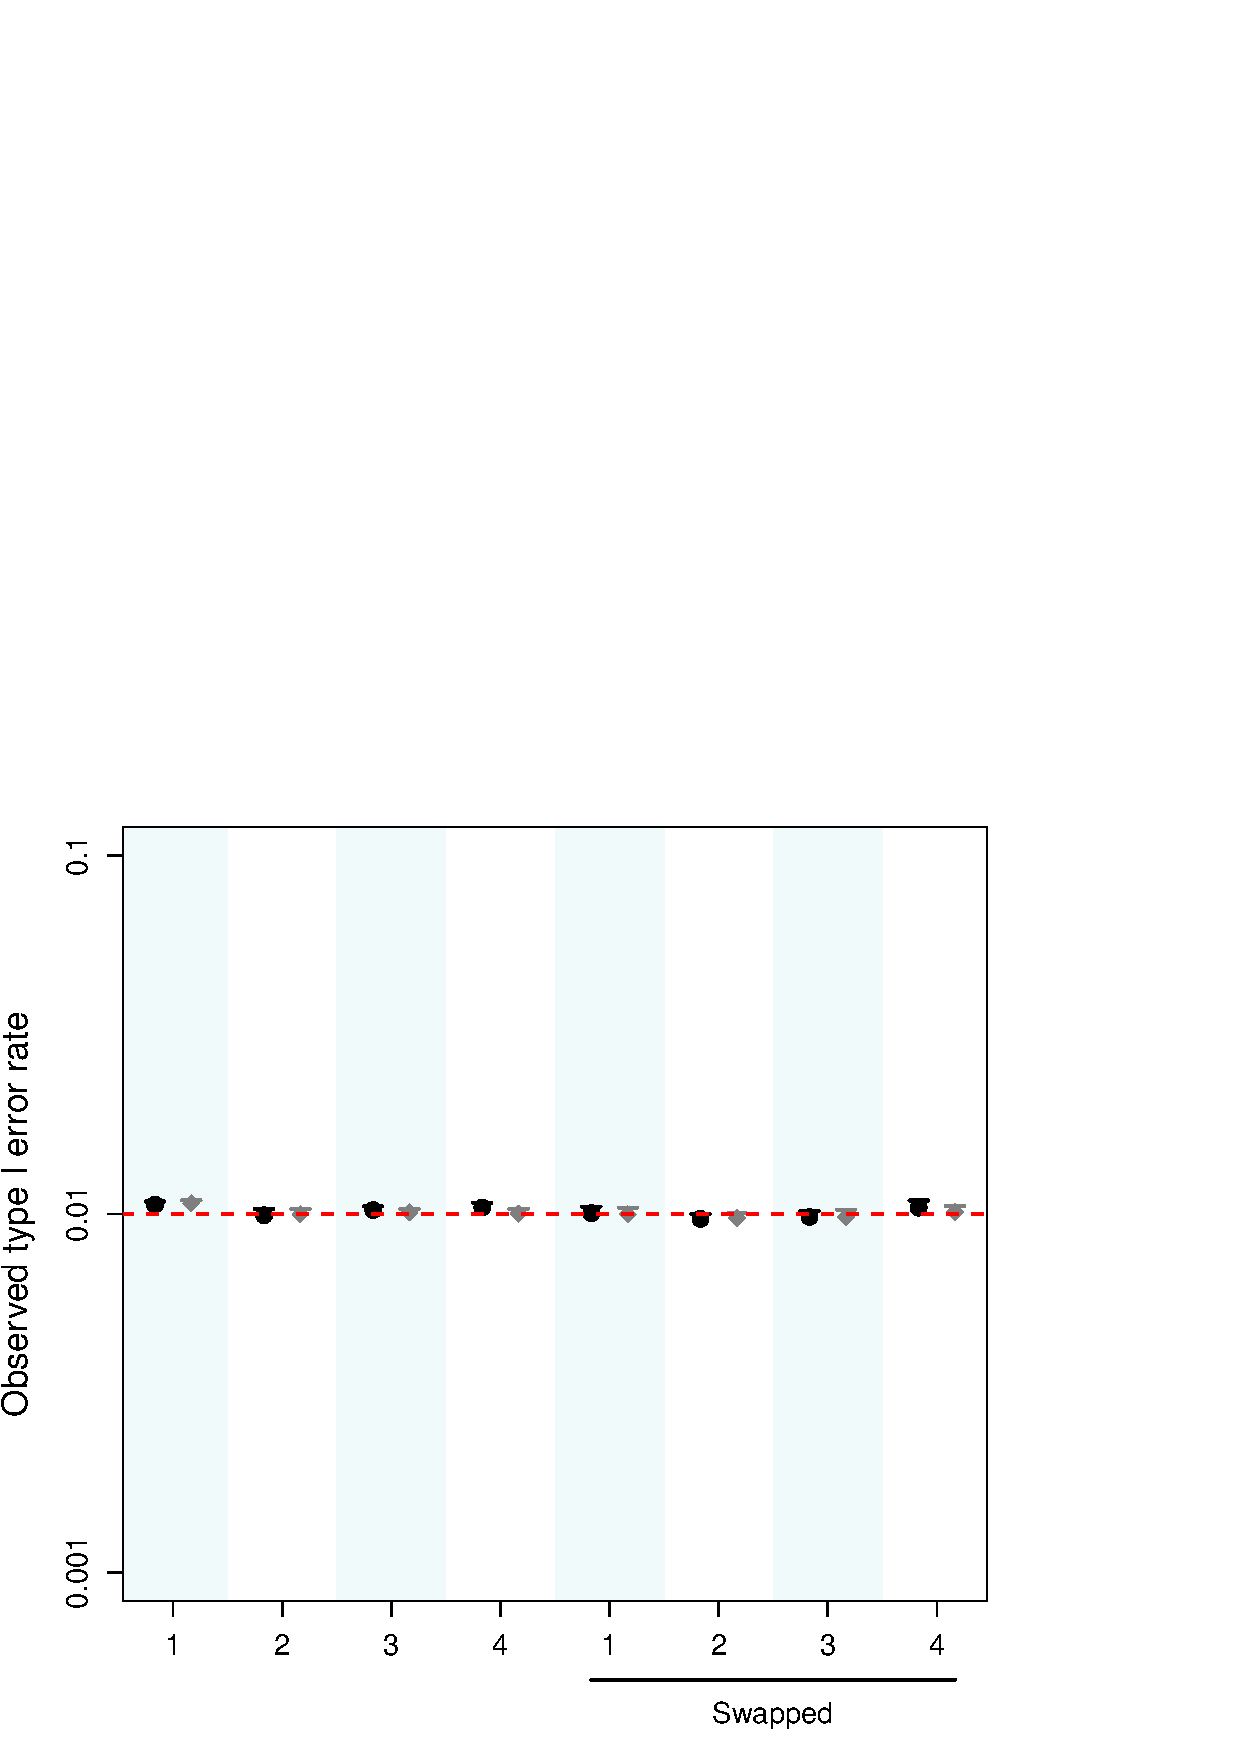
\includegraphics[width=0.48\textwidth,trim=0mm 0mm 0mm 10mm,clip]{quantile_with.pdf}
\includegraphics[width=0.48\textwidth,trim=0mm 0mm 0mm 10mm,clip]{quantile_without.pdf}
\end{center}
\caption{
    Observed type I error rates for each method on simulated data, with direct summation (black circles) and summation of quantile-adjusted pseudo-counts (grey diamonds). 
    Simulations were performed in the presence (left) or absence (right) of a plate effect, for a number of scenarios
        -- differing numbers of cells per plate (1);
        small (2), moderate (3) or large differences (4) in library size within plates;
        as well as the corresponding scenarios where plates were swapped between conditions.
    Error rates are shown on a log scale and represent the average across 10 simulation iterations.
    Each error bar represents the standard error of the corresponding log-average rate.
    The threshold of 0.01 is represented by the red dotted line.
}
\label{fig:complexplate}
\end{figure}

\section{Summation results in reduced DE detection in real data}
The simulations suggest that DE analyses on summed counts are less liberal than analyses using the original single-cell counts.
To determine whether this behaviour is relevant, both strategies were applied on real data from two scRNA-seq studies.
The first study examines mouse embryonic stem cells (mESCs) cultured under three different serum conditions \cite{kolod2015single},
    where all mESCs on each C1 chip correspond to a single condition (serum, 2i, or the alternative ground state a2i).
The second study examines gastrulation in the early mouse embryo at various development stages \cite{scialdone2015single},
    where all cells on each plate originate from the same stage.

For the first study, count data was obtained from \url{http://www.ebi.ac.uk/teichmann-srv/espresso}. 
This data set contains multiple chips across several batches for each serum condition.
Counts were only taken from the two batches where all three serum conditions were represented.
To account for the batch effect, the experimental design was parametrized as an additive model with serum-specific expression terms and batch-specific blocking factors.
For the second study, data was obtained from \url{http://www.ebi.ac.uk/antonio/some-silly-pun}.
Counts were taken from a subset of cells in the primitive streak (PS) and neural plate (NP) stages.
This subset contains all cells used in Figure X in \cite{scialdone2015single}, and was originally selected by clustering on the single-cell expression profiles 
    -- this is slightly conservative as cells with DE are less likely to be included in that cluster.
A one-way layout was then used to model the two stages, with two plates per stage.

% Note that Kim used ComBat to remove batch effects, not plate effects.
% Trying to do so won't work; ComBat will fail because it recognises (rightfully) that the plate effect is confounding with the conditions in the design matrix.
% In any case, ComBat seems to just regress out the plate effect, so even if you gave an all-intercept matrix to get it to run, you'd lose all DE.

DE analyses were performed on each data set with DESeq2, voom or the QL framework in edgeR.
These methods were chosen as they could be applied on both the single-cell counts and summed counts for all cells in each plate. 
Analyses were performed to detect DE genes between 2i and serum in the first study; between a2i and serum; and between the PS and NP stages in the second study.
%In each data set, low-quality cells were removed if they had library sizes below 10$^5$ reads or more than 10\% of reads assigned to mitochondrial genes.
Low-abundance genes were defined as those with an average count below 1 across all cells and were filtered out.
Each analysis method was then implemented as previously described. 
Sample-level quality control was not applied as low-quality cells had already been removed.
The total number of DE genes detected at a FDR of 5\% was counted for each method, with and without summation.
The number of DE genes detected in both approaches was also counted.

In all comparisons, the number of DE genes detected with summed counts was substantially smaller than that detected with single-cell counts (Table~\ref{tab:realnum}).
The DE list from the latter was a superset of that from the former.
However, this does not mean that the DE analyses with single-cell counts provide more power.
Recall that the single-cell analyses fail to maintain type I error control in the simulations.
This suggests that the increased numbers in Table~\ref{tab:realnum} correspond to detection of false positives rather than genuine DE genes.
Conversely, reduced detection of DE genes by the analyses on summed counts is consistent with more accurate error control.
It should be stressed that differences in the number of DE genes can only be interpreted as a difference in power when the number of false positives are similar.
This is clearly not the case here -- the previous simulations demonstrate that the analyses on single-cell counts are substantially liberal.

\begin{table}[btp]
\caption{Total number of DE genes detected by each method in each comparison at a FDR of 5\%, using the single-cell or summed counts.
The number of DE genes detected with both counts is also shown.
}
\label{tab:realnum}
\begin{center}
\begin{tabular}{l l r r r}
\hline
\textbf{Comparison} & \textbf{Counts} & \textbf{DESeq2} & \textbf{voom} & \textbf{edgeR} \\
\hline
\multirow{3}{*}{2i vs. serum} 
& Cell & 7419 & 9585 & 7127 \\
& Sum & 3227 & 1691 & 946 \\
& Shared & 2948 & 1678 & 946 \\
\hline
\multirow{3}{*}{a2i vs. serum} 
& Cell & 6447 & 9202 & 6013 \\
& Sum & 2004 & 758 & 238 \\
& Shared & 1876 & 747 & 238 \\
\hline
\multirow{3}{*}{PS vs. NP} 
& Cell & 268 & 4862 & 522 \\
& Sum & 17 & 0 & 0 \\
& Shared & 15 & 0 & 0 \\
\hline
\end{tabular}
\end{center}
\end{table}

To determine the effect of summation on the gene ranking, genes were sorted based on the $p$-value computed from each method.
The identities of the top 20, 200 and 2000 genes were compared for analyses using single-cell and summed counts.
In general, less than half of the top-ranking genes are shared between the two analyses for each method (Table~\ref{tab:realrank}).
The difference is attributable to changes in variance modelling after summation, to focus on variability between plates rather than between cells.
This effect is important as genes associated with phenotypic differences between conditions are expected to exhibit strong DE.
Thus, the top-ranking genes are typically prioritized for further interpretation and investigation.
Changes to the ranking indicate that summation will affect the biological conclusions that are taken from the analysis.

\begin{table}[btp]
\caption{Proportion of the top-ranking DE genes shared between analyses using the single-cell or summed counts.
Top genes were defined as those with the smallest 20, 200, or 2000 $p$-values in each comparison.
}
\label{tab:realrank}
\begin{center}
\begin{tabular}{l l r r r}
\hline
\textbf{Comparison} & \textbf{Top} & \textbf{DESeq2} & \textbf{voom} & \textbf{edgeR} \\
\hline
\multirow{3}{*}{2i vs. serum} 
& 20 & 0.10 & 0.05 & 0.20 \\
& 200 & 0.25 & 0.43 & 0.35 \\
& 2000 & 0.49 & 0.60 & 0.60 \\
\hline
\multirow{3}{*}{a2i vs. serum} 
& 20 & 0.30 & 0.15 & 0.20 \\
& 200 & 0.26 & 0.54 & 0.31 \\
& 2000 & 0.46 & 0.58 & 0.61 \\
\hline
\multirow{3}{*}{PS vs. NP} 
& 20 & 0.35 & 0.30 & 0.35 \\
& 200 & 0.30 & 0.26 & 0.44 \\
& 2000 & 0.39 & 0.26 & 0.66 \\
\hline
\end{tabular}
\end{center}
\end{table}

One potential criticism of summation is that the variability between cells is hidden in the count sum.
One might expect that genes with DE driven by a few outlier cells would be ranked highly, as they would no longer be penalized by a large cell-to-cell variance estimate.
This would not be appropriate as such outlier patterns are uninteresting.
However, these genes do not seem to be favoured in real data.
Figure~\ref{fig:realdata} shows the top set of DE genes from summation, all of which exhibit robust differences between conditions.
DE genes driven by a few outliers tend to be less significant.
This is because the conditional variance of the count sum increases with fewer contributing cells, 
    which increases the total variance and decreases the relative significance of DE.
Technical noise and heterogeneity will no longer average out when the sum consists of very few cells.

\begin{figure}[bt]
    \begin{center}
        \includegraphics[width=\textwidth]{realdata_top_edgeR_ola1_sum.pdf}
        \includegraphics[width=\textwidth]{realdata_top_edgeR_ola2_sum.pdf}
    \end{center}
\caption{
    Expression profiles of DE genes between 2i and serum (top) or between a2i and serum conditions (bottom) in the mESC data set, 
        for the top genes detected by QL edgeR on summed counts.
    Each plot contains the expression profile for one gene, where the $y$-axis represents the log-CPMs.
    Each point represents a cell in the serum (black) or a2i/2i conditions (grey).
    A prior of 0.25 was added to each count to avoid undefined log-CPMs from zeroes.
    For simplicity, only cells in one batch are shown for both contrasts.
}
\label{fig:realdata}
\end{figure}

% The second kolod comparison is the only one with decent DE for all methods,
% which is why it's being used here.

\section{Conclusions}
Confounding plate effects are often present in scRNA-seq data sets, but are typically ignored during the DE analysis.
Simulations indicate that this strategy is not statistically rigorous and will result in loss of type I error control. 
In this article, a solution is presented involving the summation of counts across all cells on each plate for each gene.
The count sums can then be used in a DE analysis, effectively treating plates as individual samples.
This restores type I error control and avoids the detection of excessive false positives.
Variance adjustment of the counts is not required prior to summation, even when the numbers or sizes of cells differ across or within plates.
Summation prior to DE analyses also affects the biological conclusions for real scRNA-seq studies, 
    by decreasing the size of the DE lists and by changing the ranking of DE genes.

It is possible to resolve plate effects at the single-cell level with careful experimental design.
In particular, cells should be arranged such that each plate contains cells from multiple conditions.
DE comparisons can then be performed within plates such that any plate effect cancels out between conditions on the same plate.
For such experimental designs, summation has fewer benefits.
This is because the biological condition is no longer confounded by the plate of origin.
The latter can be included as a blocking factor in the linear model for the single-cell counts, 
    to explicitly regress out the plate effect without removing genuine DE between conditions.
This avoids any loss of type I error due to hidden correlations between cells on each plate.

Nonetheless, summation can still be applied to all cells of the same condition on each plate.
This increases the count sizes and decreases technical noise for greater compatibility with existing analysis methods like edgeR.
It also reduces computational work as the sample size is defined from the number of plates ($<$ 10), not the number of cells ($>$ 100).
Power is unaffected by summation as the nature of the DE comparison (i.e., between condition averages) remains unchanged.
More generally, including several different conditions on a single plate may not always be logistically feasible, and designs with one condition per plate are often more practical.
In such cases, the best way to handle plate effects is to simply increase the number of plates.
This provides more residual d.f. to precisely estimate the plate-to-plate variability after summation.
The number of cells is less important, though there should be enough cells per plate to obtain stable count sums.

One particular benefit of using summed counts with existing analysis methods is in the normalization step.
Methods like size factor and TMM normalization are based on ratios between counts in different cells,
    but will be compromised for noisy data that contains many zero and near-zero counts.
Summation reduces the incidence of such counts so that these normalization methods can be properly applied.
Specifically, normalization of the summed counts will remove plate-specific differences that affect each gene in the same manner, 
    e.g., differences in capture efficiency or sequencing depth between plates.
Removal of cell-specific biases within each plate is not required as these will average out when many cells are summed together.
Indeed, type I error control is maintained in simulations where the library size differs across cells.

% And if it doesn't average out, then it will be considered to be a plate-specific difference and removed anyway.

Summation is a simple but effective approach to overcome the problem of plate effects in a DE analysis. 
This complements other aspects of the data analysis that use single-cell counts, e.g., in cell clustering or to identify highly variable genes.
Summation also reduces technical noise and may be a more general strategy to improve data quality when many cells are available,
    such as in droplet-based protocols \cite{klein2015droplet,macosko2015highly}.

\bibliographystyle{unsrt}
\bibliography{references}

\end{document}
